\documentclass{beamer}
\usepackage{amsmath} 
\usepackage{graphicx} 
\usepackage{color}
\usepackage[utf8]{inputenc}
\usepackage{subfigure}
\usepackage{caption}
\usepackage{bm}
\usepackage[linesnumbered,boxed]{algorithm2e}
%\captionsetup{font={scriptsize}}
\title{Monte Carlo Simulation of Two-dimensional Ising model}
\author{Tong Li}
\institute{Department of Physics \& Astronomy \\ Michigan State University }
\date{\today}
\setbeamertemplate{footline}[frame number] 
\usecolortheme{seahorse}
\setbeamertemplate{caption}[numbered]

\makeatletter
\def\blfootnote{\gdef\@thefnmark{}\@footnotetext}
\makeatother

\renewcommand{\thefootnote}{\fnsymbol{footnote}}

\begin{document}
\beamertemplatenavigationsymbolsempty

\thispagestyle{empty} 
\begin{frame}
\titlepage
\end{frame}

\begin{frame}{Outline}
\tableofcontents
\end{frame} 

\section{Introduction}	
\begin{frame}{Introduction}
\begin{itemize}
	\item <1-> Ising model is a simple but important model for the explanation of ferromagnetism.  
	\item <2-> 
	Atomic spins are located on a $N$-dimensional lattice grid, 
	and these spins only have two discrete states, up ($\sigma=1$) or down ($\sigma=-1$). 
	\item <3-> 
	Only neighboring spins can interact with each other, and thus its Hamiltonian can be written as 
	\begin{equation}\label{eq:hamiltonian}
	H=-J\sum_{<kl>}^{N}\sigma_k\sigma_l\,, 
	\end{equation}
	where $J>0$ and $<kl>$ indicates that we only sum over nearest neighbors. 
\end{itemize}
\end{frame}

\begin{frame}{Introduction}
\begin{itemize}
	\item <1-> Only one- and two-dimensional cases has been solved analytically and they show several interesting properties of phase transition. 
	\item <1-> Therefore, it is necessary to develop an efficient numerical method for the simulation of Ising model. 
	\item <2-> In this work we focus on the Monte Carlo simulation of 2D Ising model, which can be benchmarked with analytical solution. 
	\item <3-> Our numerical framework can also be easily extended to higher dimensions. 
\end{itemize}
\end{frame}

\section{Properties of 2D Ising model from its analytical solution}

\begin{frame}{Outline}
\tableofcontents[currentsection]
\end{frame}

\subsection{The solution of $2 \times 2$ Ising model}
\begin{frame}{Properties of 2D Ising model from its analytical solution}
\begin{itemize}
	\item<1-> We first solve $2 \times 2$ case with periodic boundary condition for benchmark. 
	\item<2-> Periodic boundary condition: a spin on one boundary will interact with another spin on the opposite boundary. 
	\item<3-> All possible microscopic states of $2 \times 2$ Ising model. The energy is in the unit of $J$. 
	\begin{table}
		\centering
		\begin{tabular}{cccc}
			\hline
			\hline 
			Number of spins up & Degeneracy & Energy & Magnetization \\ 
			\hline
			4 & 1 & -8 & 4 \\  
			3 & 4 & 0 & 2 \\ 
			2 & 4 & 0 & 0 \\ 
			2 & 2 & 8 & 0 \\ 
			1 & 4 & 0 & -2 \\ 
			0 & 1 & -8 & -4 \\ 
			\hline 
			\hline
		\end{tabular}
		\label{tab:2times2} 
	\end{table}
\end{itemize}
\end{frame}

\begin{frame}{The solution of $2 \times 2$ Ising model}
\begin{itemize}
	\item<1-> The partition function of canonical ensemble can be obtained by summing over all these microscopic states $\alpha$ 
	\begin{equation}
	Z=\sum_{\alpha}e^{-\beta E_\alpha}=2e^{8\beta}+2e^{-8\beta}+12=4\cosh\left(8\beta\right)+12\,,
	\end{equation}
	where $\beta=1/T$ and $T$ is temperature in the unit of $J$ ($k_B=1$). 
	\item<2-> The mean energy of the system (in the unit of $J$) is 
	\begin{equation}
	\langle E\rangle=-\frac{\partial \ln Z}{\partial \beta}=-\frac{8\sinh\left(8\beta\right)}{\cosh\left(8\beta\right)+3}\,. 
	\end{equation}
	The mean magnetization of the system is 
	\begin{equation}
	\langle|M|\rangle=\frac{1}{Z}\sum_{\alpha} |M_\alpha| e^{-\beta E_\alpha}=\frac{1}{Z}\left(8e^{8\beta}+4\right)
	=\frac{2e^{8\beta}+1}{\cosh\left(8\beta\right)+3}\,. 
	\end{equation}
\end{itemize}
\end{frame}

\begin{frame}{The solution of $2\times 2$ Ising model}
\begin{itemize}
	\item<1-> 	The heat capacity is 
	\begin{equation}\label{eq:cv}
	C_V=\frac{\partial \langle E\rangle}{\partial T}=-\beta^2\frac{\partial \langle E\rangle}{\partial \beta}
	=\beta^2\frac{64\left[1+\cosh\left(8\beta\right)\right]}{\left[6+\cosh\left(8\beta\right)\right]^2}
	\,. 
	\end{equation}
	\item<2-> Also it can be proved that for any system under canonical ensemble 
	\begin{equation}
	C_V=\beta^2\left(\langle E^2\rangle-\langle E\rangle^2\right)\,,
	\end{equation}
	where for $2\times 2$ case 
	\begin{equation}
	\langle E^2\rangle=\frac{1}{Z}\sum_{\alpha}E^2_\alpha e^{-\beta E_\alpha}=\frac{64\cosh\left(8\beta\right)}{\cosh\left(8\beta\right)+3}\,. 
	\end{equation}
	\item<2-> 
	Similarly, we have 
	\begin{equation}
	\langle M^2\rangle=\frac{1}{Z}\sum_{\alpha} M^2_\alpha e^{-\beta E_\alpha}=\frac{8\left(e^{8\beta}+1\right)}{\cosh\left(8\beta\right)+3}\,, 
	\end{equation}
	and define susceptibility as 
	\begin{equation}\label{eq:chi}
	\chi=\beta\left(\langle M^2\rangle -\langle |M|\rangle ^2\right)\,. 
	\end{equation}
\end{itemize}
\end{frame}

\subsection{Properties of phase transition in 2D Ising model}
\begin{frame}{Properties of phase transition in 2D Ising model}
\begin{itemize}
	\item<1-> One interesting aspect of 2D (and higher dimensional) Ising model is the second-order phase transition 
	at a nonzero critical temperature $T_C$. 
	\item<2-> There is a sharp transition from nonzero $\langle|M|\rangle $ (ordered phase) to $\langle|M|\rangle=0$ (disordered phase)
	when temperature $T$ increases from $T<T_C$ to $T>T_C$. 
	\item<3-> According to the analytical solution of 2D Ising model, the mean magnetization is given by
	\begin{equation}
	\langle M(T) \rangle \sim \left(T-T_C\right)^{\beta}\,,
	\end{equation}
	where $\beta=1/8$ is a critical exponent. Similarly heat capacity satisfies 
	\begin{equation}
	C_V(T) \sim \left|T_C-T\right|^{\alpha}\,,
	\end{equation}
	and the susceptibility 
	\begin{equation}
	\chi(T) \sim \left|T_C-T\right|^{\gamma}\,,
	\end{equation}
	with $\alpha = 0$ (logarithmic divergence) and $\gamma = 7/4$. 
\end{itemize}
\end{frame}

\begin{frame}{Properties of phase transition in 2D Ising model}
\begin{itemize}
	\item<1-> A second-order phase transition is characterized by a
	correlation length $\xi$ that spans the whole system. 
	\item<2-> When $T>>T_C$, spins orient randomly without correlation, and $\xi$ is of the order of lattice spacing. 
	\item<3-> Spins	become more and more correlated as $T$ goes down and approaches $T_C$, 
	$\xi$ increases significantly. \\ The divergent
	behavior of $\xi$ near $T_C$ is 
	\begin{equation}
	\xi(T) \sim \left|T_C-T\right|^{-\nu}\,,
	\label{eq:xi}
	\end{equation}
	with $\nu=1$ given by the analytical solution. 
	\item<4-> Because we are limited to a finite lattice, $\xi$ will
	be proportional with the size of the lattice when phase transition occurs. 
	\item<5-> Through finite size scaling relation 
	we get the critical temperature that scales as
	\begin{equation}
	T_C(L)-T_C(L=\infty) = aL^{-1/\nu}\,,
	\end{equation}
	where $a$ is a constant and $\nu$ is defined in Eq. \ref{eq:xi}. 
\end{itemize}
\end{frame}

\section{Monte Carlo methods for Ising model}
\begin{frame}{Outline}
\tableofcontents[currentsection]
\end{frame}

\begin{frame}{Monte Carlo methods for Ising model}
\begin{itemize}
	\item<1-> We use Metropolis algorithm based on the theory of Markov chain and detailed balance. 
	\item<2-> The transition rate between two microscopic states $i$ and $j$ should satisfy 
	\begin{equation}\label{eq:Wfrac}
	\frac{W(j \rightarrow i)}{W(i \rightarrow j)}=\frac{w_i}{w_j}=e^{-\beta\left(E_i-E_j\right)}\,,
	\end{equation}
	with $w_i=\frac{1}{Z}e^{-\beta E_i}$ 
	\item<3-> 
	\begin{equation}
	W(j \rightarrow i)=T(j \rightarrow i)A(j \rightarrow i)\,.
	\end{equation}
	\item<4-> We have no physical insight of $T(j \rightarrow i)$, 
	so we simply assume that all $T(j \rightarrow i)$ are the same. 
	\item<5-> 
	\begin{equation}\label{eq:Afrac}
	\frac{A(j \rightarrow i)}{A(i \rightarrow j)}=e^{-\beta\left(E_i-E_j\right)}\,,
	\end{equation}
	which describes the probability of accepting a transition from $j$ to $i$ in our simulation. 
\end{itemize}
\end{frame}

\begin{frame}
\centering
\scalebox{.68}{
	\begin{algorithm}[H]
		\caption{Metropolis algorithm for the simulation of Ising model. }
		\label{alg::metropolis}
		\KwIn{Size of the system $L$, temperature $T$, number of Monte Carlo cycles $MC$. }
		\KwOut{$\langle E \rangle$, $\langle E^2 \rangle$, $\langle |M| \rangle$, $\langle M^2 \rangle$, $C_V$ and $\chi$. } 
		Initialize spin lattice $a$ (in an ordered or random way)\;
		Calculate $E$, $E^2$, $|M|$, $M^2$ of the initial lattice\; 
		$E_{tot}=0,\,E^2_{tot}=0,\,|M|_{tot}=0,\,M^2_{tot}=0$\;
		\For{$i=1;i<=MC;i++$}
		{
			\For{$j=1;j<=L;j++$}
			{
				\For{$k=1;k<=L;k++$}
				{
					$r=$ a uniformly distributed random number in $[0,1]$\;
					Flip spin at position $(j,k)$\;
					Calculate the change of energy $\Delta E$\; 
					\If{$\Delta E < 0\ \mathrm{or}\ r<\exp\left(-\Delta E/T\right)$}
					{
						Accept this spin flip\; 
						Update $E$, $E^2$, $|M|$, $M^2$\;
					}
					\Else
					{
						Reverse this spin flip\;
					}
					Add $E$, $E^2$, $|M|$, $M^2$ to their corresponding ``tot" variables\; 
				}
			}
		}
		Calculate $\langle E \rangle$, $\langle E^2 \rangle$, $\langle |M| \rangle$, $\langle M^2 \rangle$ by dividing $L^2MC$\; 
		Calculate $C_V$ and $\chi$\;
	\end{algorithm}
}
\end{frame}

\section{Results and discussion}
\begin{frame}{Outline}
\tableofcontents[currentsection]
\end{frame}

\subsection{Results of $2 \times 2$ case}
\begin{frame}{Results of $2 \times 2$ case}
\begin{table}
	\centering
	\caption{Results for $2\times2$ case with temperature $T=1.0$. Analytical results are provided for benchmark. 
		Energy is in the unit of $J$. }
	\begin{tabular}{cccccc}
		\hline
		\hline
		$MC$ & 10 & 100 & 1000 & 10000 & Analytical \\ 
		\hline
		$\langle E \rangle$ & -7.2 & -7.92 & -7.986 & -7.988 & -7.98393\\ 
		$\langle |M| \rangle$ & 3.75 & 3.975 & 3.9955 & 3.99625 & 3.99263\\ 
		$\langle E^2 \rangle$ & 57.6  & 63.36 & 63.888 & 63.904 & 63.8714\\ 
		$\langle M^2 \rangle$ & 14.7 & 15.87 & 15.977 & 15.9805 & 15.9732\\ 
		$C_V$ & 5.76 & 0.6336 & 0.111804 & 0.095856 & 0.128329\\ 
		$\chi$ & 0.6375 & 0.069375 & 0.0129798 & 0.0104859 & 0.0320873\\ 
		\hline
		\hline 
	\end{tabular} 
	\label{tab:2times2result}
\end{table}
\end{frame}

\subsection{Convergence and probability distribution}
\begin{frame}{Convergence and probability distribution}
\begin{figure}
	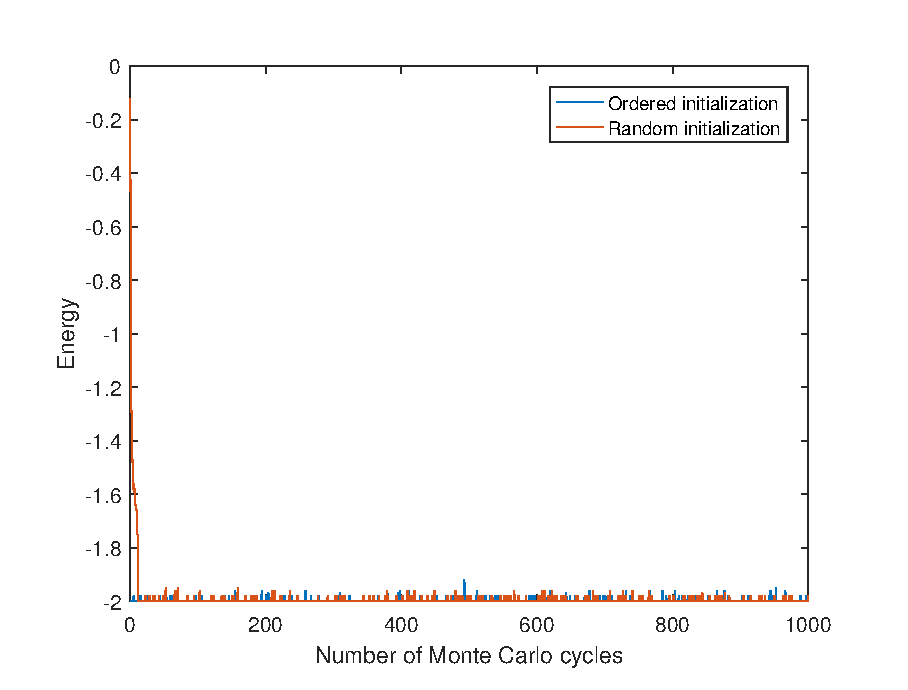
\includegraphics[width=0.8\textwidth]{Process_ene_lowT.eps}
	\caption{Energy as a function of the number of Monte Carlo cycles for $T=1.0$, $L=20$. }
\end{figure}
\end{frame}

\begin{frame}{Convergence and probability distribution}
\begin{figure}
	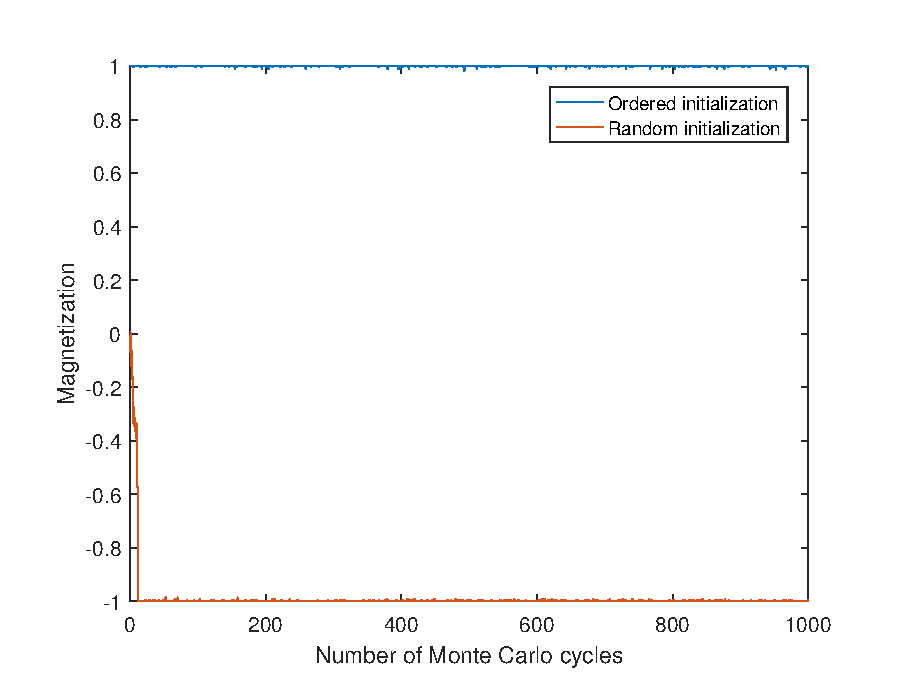
\includegraphics[width=0.8\textwidth]{Process_mag_lowT.eps}
	\caption{Magnetization as a function of the number of Monte Carlo cycles for $T=1.0$, $L=20$. }
\end{figure}
\end{frame}

\begin{frame}{Convergence and probability distribution}
\begin{figure}
	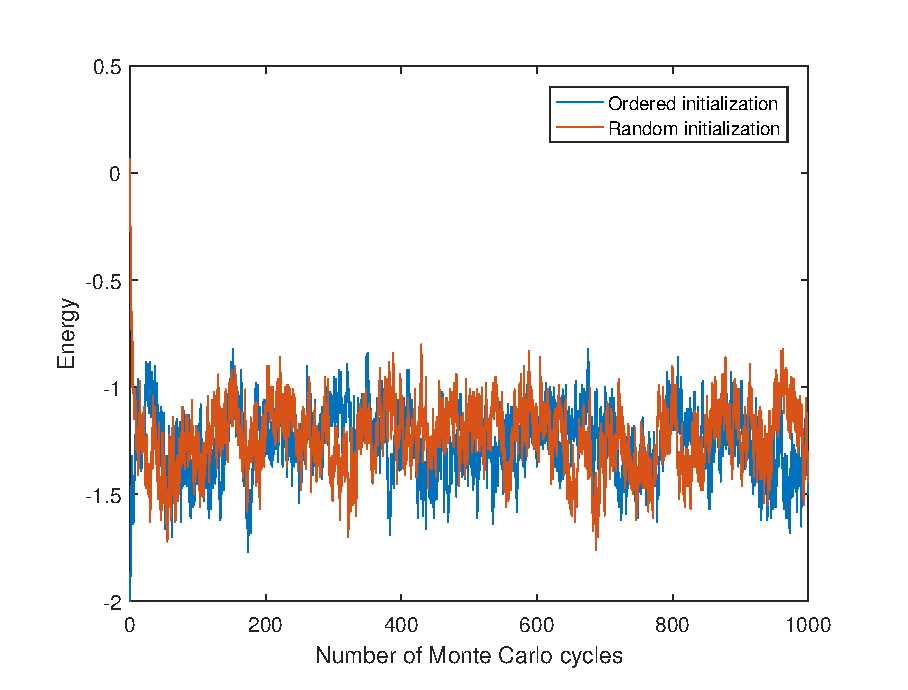
\includegraphics[width=0.8\textwidth]{Process_ene_highT.eps}
	\caption{Energy as a function of the number of Monte Carlo cycles for $T=2.4$, $L=20$. }
\end{figure}
\end{frame}

\begin{frame}{Convergence and probability distribution}
\begin{figure}
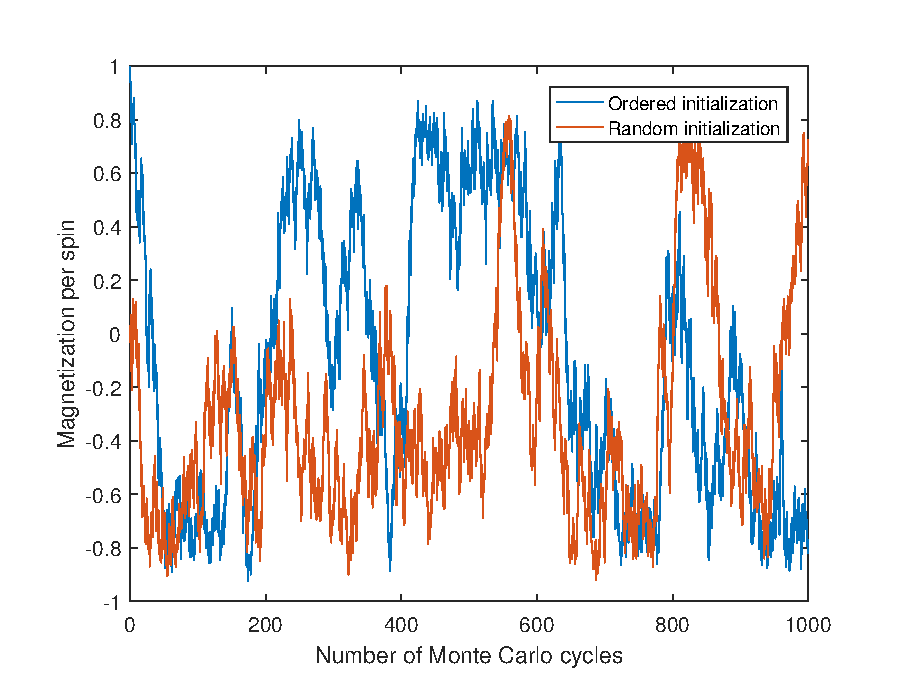
\includegraphics[width=0.8\textwidth]{Process_mag_highT.eps}
\caption{Magnetization as a function of the number of Monte Carlo cycles for $T=2.4$, $L=20$. }
\end{figure}
\end{frame}

\begin{frame}{Convergence and probability distribution}
\begin{figure}
	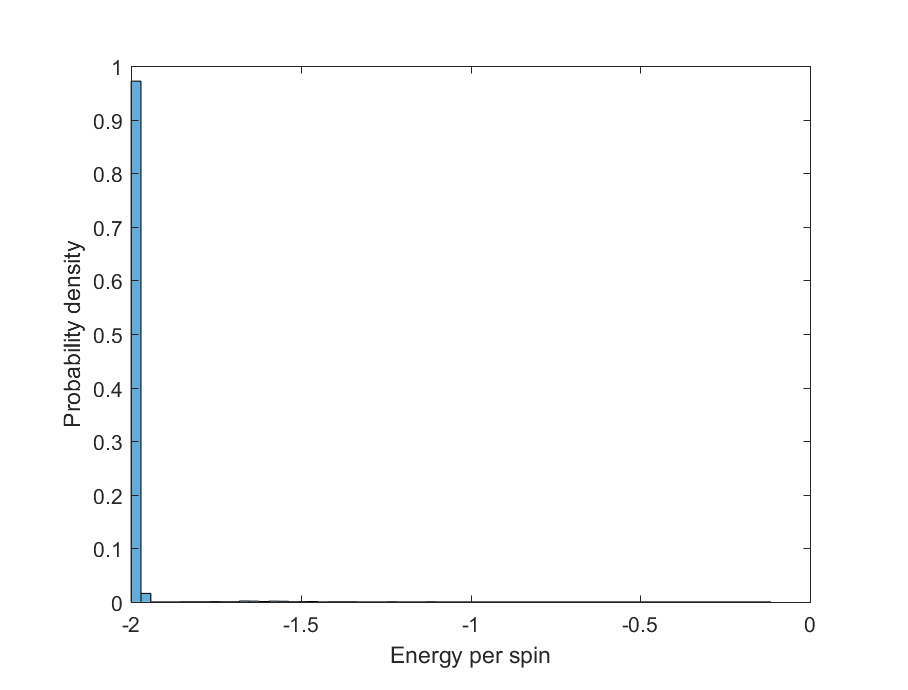
\includegraphics[width=0.8\textwidth]{Prob_ene_lowT.eps}
	\caption{Distribution of energy for $T=1.0$, $L=20$. }
\end{figure}
\end{frame}

\begin{frame}{Convergence and probability distribution}
\begin{figure}
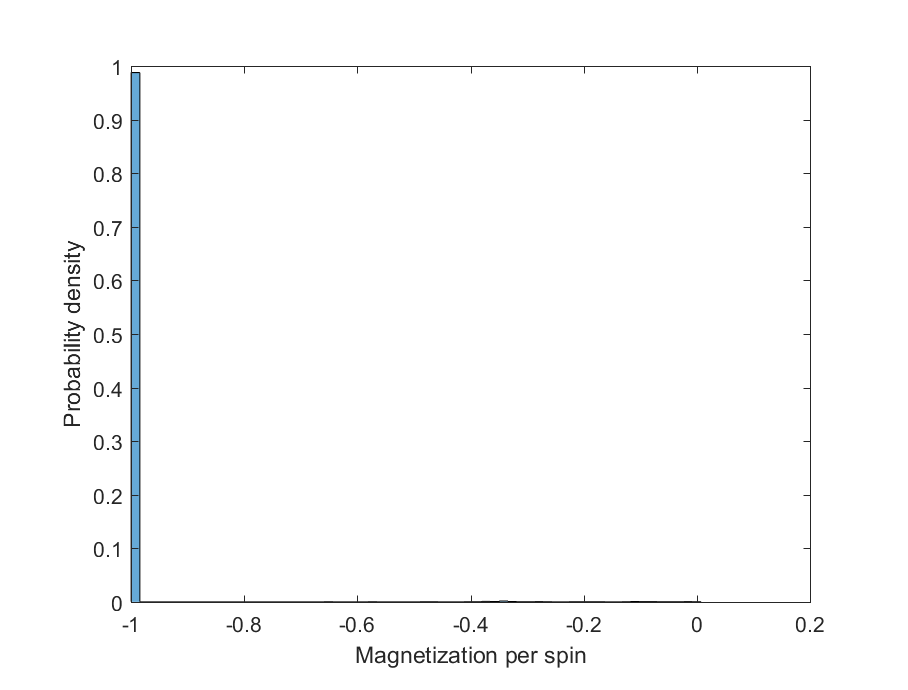
\includegraphics[width=0.8\textwidth]{Prob_mag_lowT.eps}
\caption{Distribution of magnetization for $T=1.0$, $L=20$. }
\end{figure}
\end{frame}

\begin{frame}{Convergence and probability distribution}
\begin{figure}
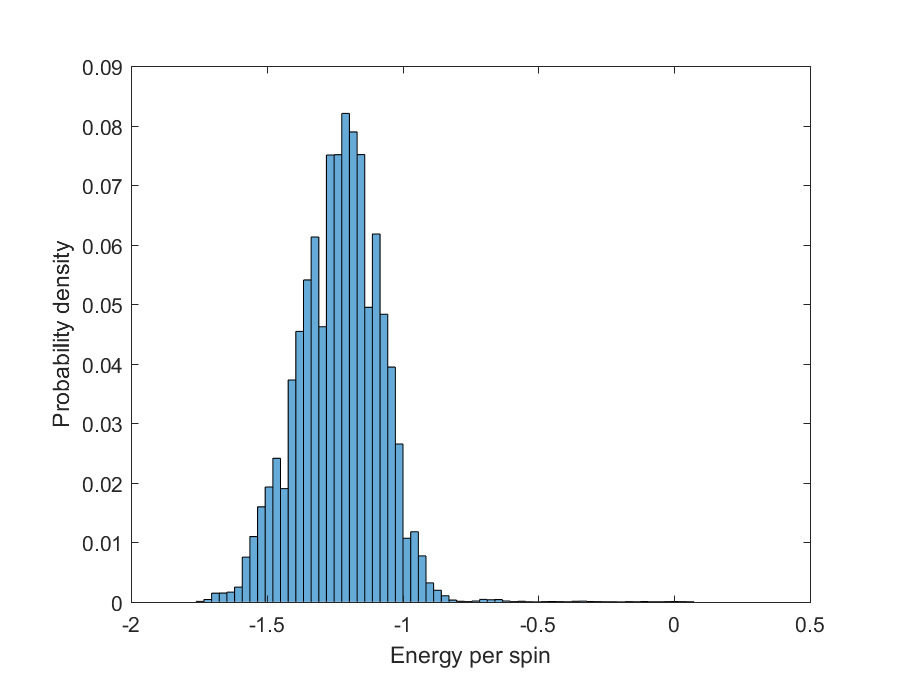
\includegraphics[width=0.8\textwidth]{Prob_ene_highT.eps}
\caption{Distribution of energy for $T=2.4$, $L=20$. }
\end{figure}
\end{frame}

\begin{frame}{Convergence and probability distribution}
\begin{figure}
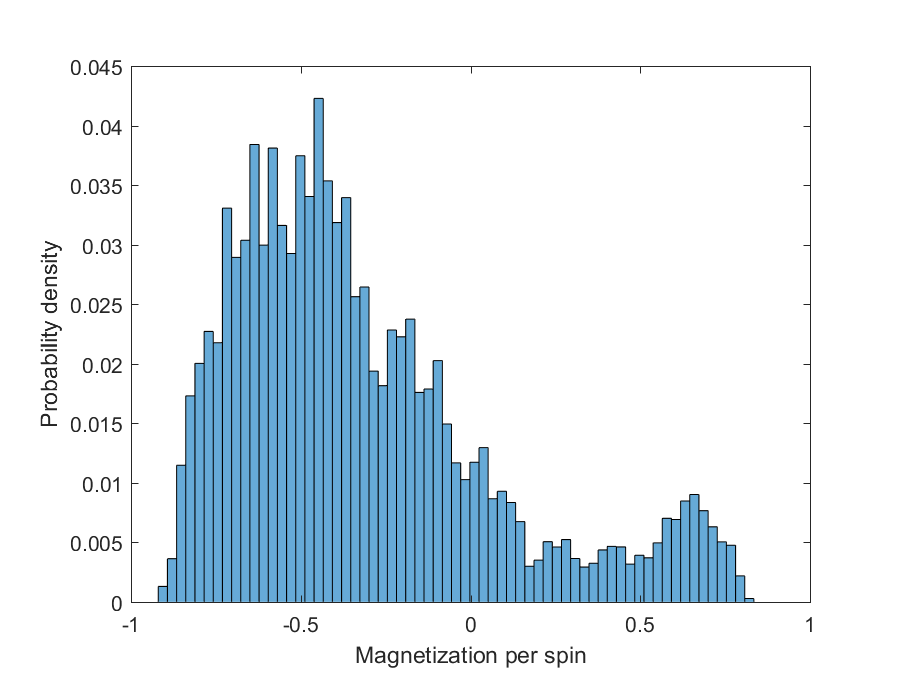
\includegraphics[width=0.8\textwidth]{Prob_mag_highT.eps}
\caption{Distribution of magnetization for $T=2.4$, $L=20$. }
\end{figure}
\end{frame}

\subsection{Phase transition}
\begin{frame}{Phase transition}
\begin{figure}
	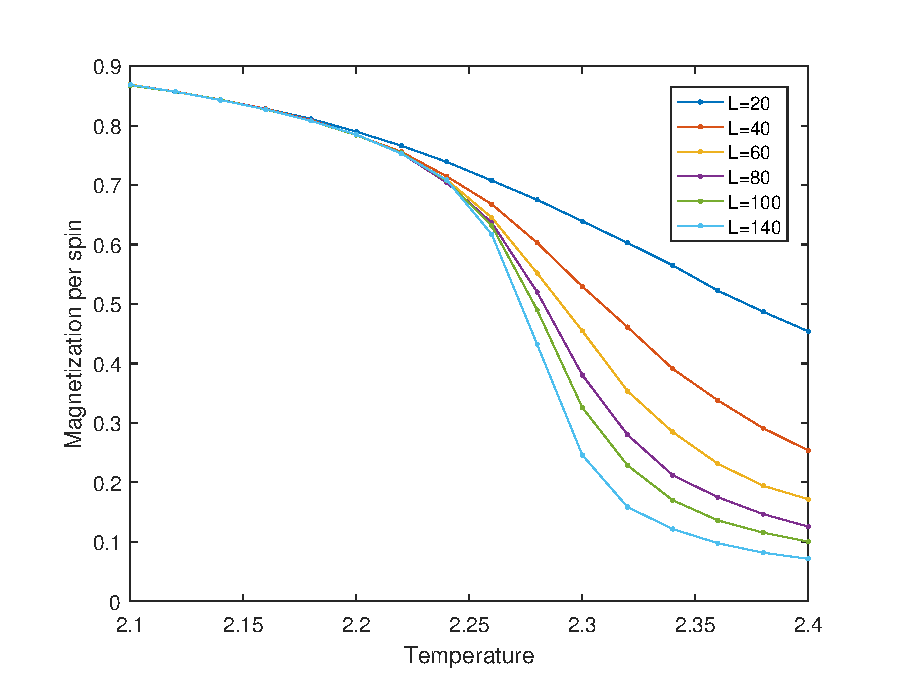
\includegraphics[width=0.8\textwidth]{Tran_mag.eps}
	\caption{Magnetization per spin as a function of temperature. Temperature step is 0.02 and the number of Monte Carlo cycles is $10^6$.  }
\end{figure}
\end{frame}

\begin{frame}{Phase transition}
\begin{figure}
	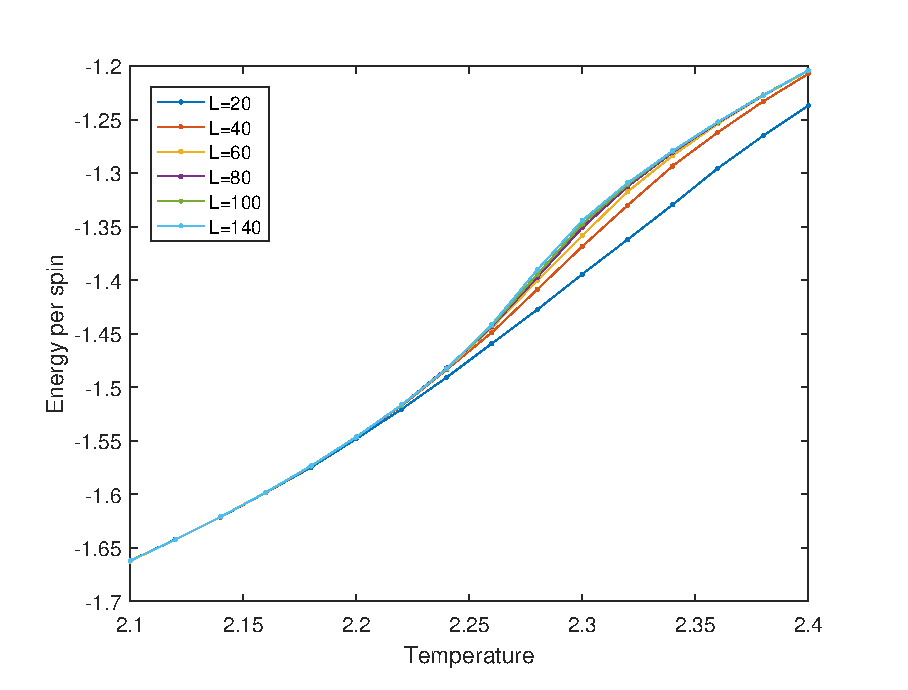
\includegraphics[width=0.8\textwidth]{Tran_ene.eps}
	\caption{Energy per spin as a function of temperature. Temperature step is 0.02 and the number of Monte Carlo cycles is $10^6$.  }
\end{figure}
\end{frame}

\begin{frame}{Phase transition}
\begin{figure}
	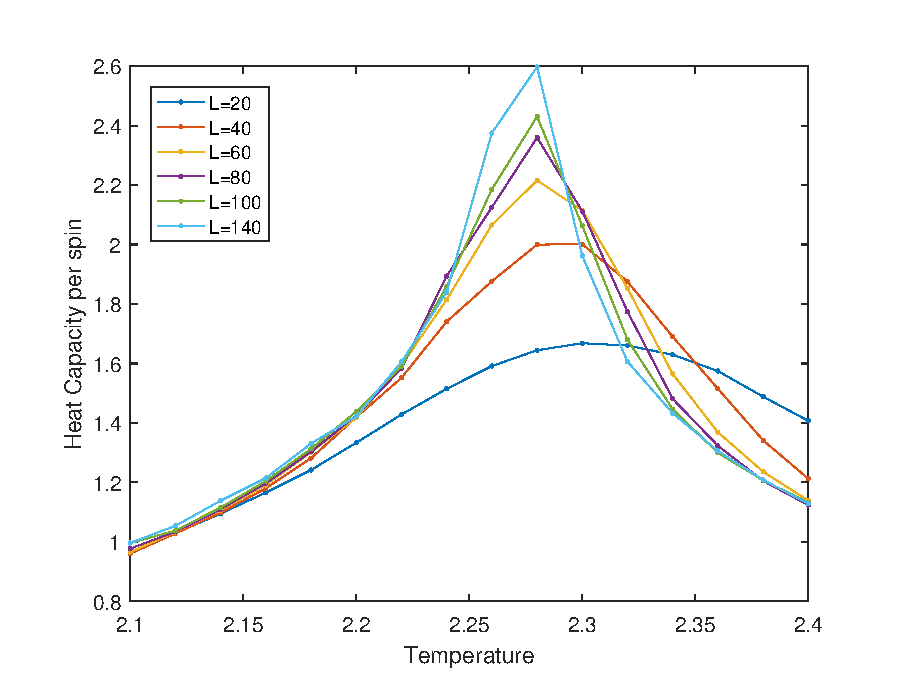
\includegraphics[width=0.8\textwidth]{Tran_Cv.eps}
	\caption{Heat capacity per spin as a function of temperature. Temperature step is 0.02 and the number of Monte Carlo cycles is $10^6$.  }
\end{figure}
\end{frame}

\begin{frame}{Phase transition}
\begin{figure}
	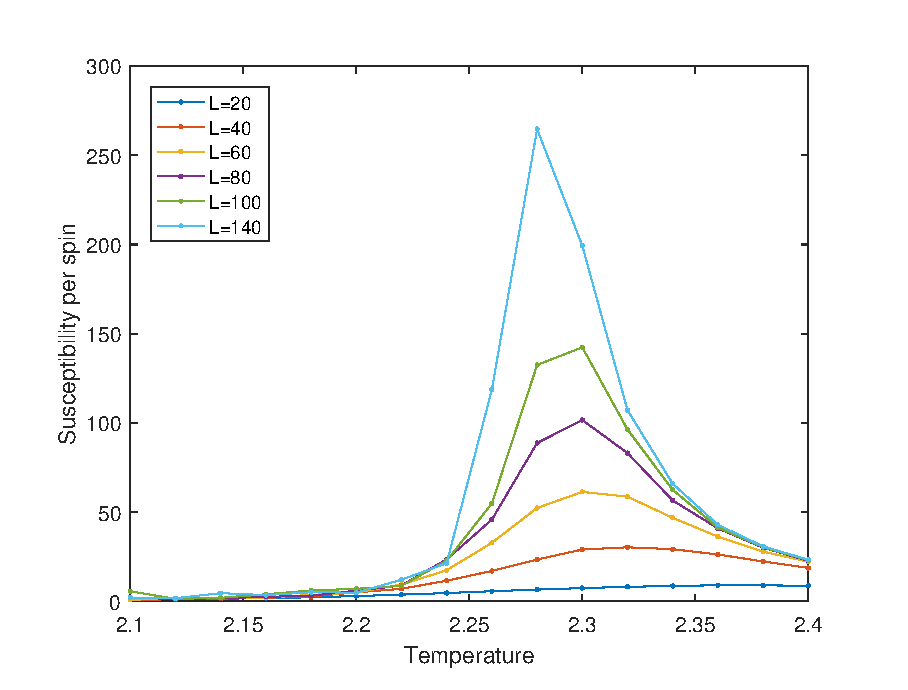
\includegraphics[width=0.8\textwidth]{Tran_sus.eps}
	\caption{Susceptibility per spin as a function of temperature. Temperature step is 0.02 and the number of Monte Carlo cycles is $10^6$.  }
\end{figure}
\end{frame}

\begin{frame}{Estimation of critical temperature}
\begin{itemize}
\item<1-> By the following equation 
\begin{equation}
T_C(L)-T_C(L=\infty) = aL^{-1/\nu}\,,
\label{eq:tc}
\end{equation}
where $a$ is a constant and $\nu=1$, 
we can estimate $T_C$ for an infinitely large system from the results with finite $L$. 
\item<2->
It is quite difficult to determine the critical temperature from previous figures 
because our resolution is not small enough. 
\item<3->
From the peaks of $\chi$ we estimate that $T_C(L=60)=2.3$ and $T_C(L=140)=2.28$. 
Then we obtain 
\begin{equation}
\left\{
\begin{array}{c}
a=2.1\,,  \\
T_C(L=\infty)=2.265\,.  \\
\end{array}
\right.
\end{equation}
\item<4-> Our estimation is close to the analytical result 2.269.
\end{itemize}
\end{frame}

\section{Conclusions}
\begin{frame}{Outline}
\tableofcontents[currentsection]
\end{frame}

\begin{frame}{Conclusions}
\begin{itemize}
	\item<1-> Our numerical results of $L=2$ case agrees well with the analytical values, 
	and calculations of $L=20$ case to confirm that the system converges fast to equilibrium in the simulation. 
	\item<2-> As expected the energy distribution centers around the mean value and a higher temperature leads to a broader distribution. 
	\item<3-> In phase transition, the behaviors of different physical quantities agree well with the analytical solution. 
	\item<4-> From the peak of susceptibility we estimate that the critical temperature for infinitely large lattice is 2.265, 
	which is close to the analytical value 2.269. 
	\item<5-> This work provides a powerful tool for the simulation of 2D Ising model, which can be extended to three-dimensional case. 
\end{itemize}
\end{frame}

\section*{References}
\begin{frame}{References}
\nocite{*} 
\scriptsize
\bibliographystyle{unsrt}
\bibliography{proj4_ref}
\end{frame}

\section*{Acknowledgment}
\begin{frame}{Acknowledgment}
	I am grateful for the sincere guidance from Prof. Morten Hjorth-Jensen. 
	\par
	Thanks for your attention! Any question? 
\end{frame}

\end{document}
